\documentclass[10pt,a4paper]{article}
\usepackage[margin=2.2cm]{geometry}
\usepackage{fontspec}
\usepackage{kotex}
\setmainfont{Apple SD Gothic Neo}
\setsansfont{Apple SD Gothic Neo}
\usepackage{amsmath,amssymb}
\usepackage{graphicx}
\usepackage{booktabs}
\usepackage{caption}
\usepackage[dvipsnames]{xcolor}
\usepackage[colorlinks=true,linkcolor=MidnightBlue,citecolor=MidnightBlue,
            urlcolor=MidnightBlue]{hyperref}
\usepackage{titlesec}
\titleformat{\section}{\large\bfseries}{\thesection}{0.6em}{}
\titleformat{\subsection}{\normalsize\bfseries}{\thesubsection}{0.5em}{}
\captionsetup{font=small,labelfont=bf}
\setlength{\parskip}{0.35em}
\setlength{\parindent}{0pt}

\usepackage{mdframed}
\newmdenv[linewidth=0.4pt,linecolor=gray!60,backgroundcolor=gray!5,
          innertopmargin=6pt,innerbottommargin=6pt,skipabove=8pt,skipbelow=8pt]{claimbox}
\newcommand{\claim}[2]{\begin{claimbox}\textbf{주장.} #1\par\smallskip
  \textcolor{gray!70}{\textbf{반증 조건.} #2}\end{claimbox}}

\title{\bfseries 걸음 하나가 결론을 정했다\\[2pt]
\large 정보 전이장은 진짜 유보에서 지속성을 이긴다 --- 그리고 예보를 올리는 손잡이가
식별을 깬다}
\author{월드모델 실험실 · 노트 732 · 733 · 734 · 735 · 736}
\date{2026-08-06}
\begin{document}\maketitle

\section{한 줄}

T5 가 닫히면서 \textbf{텍스트 표현은 도메인 안 전용으로 확정됐다}(논문 144). 그러면
도메인을 넘는 표현으로 남은 것은 \textbf{정보 전이장} 하나다. 그것을 \textbf{진짜
유보}(목표일 $2025$-$01$-$01 \sim 2026$-$07$-$06$)로 재니 \textbf{$R^2 = +0.1200$}
이고 위약이 $-0.0027$ 이며 짝 차가 \textbf{$5.6\sigma$} 다 --- \textbf{장은 어제를
베끼는 것보다 낫다.} 그런데 그 값을 얻으려면 \textbf{걸음 수를 고쳐야 했고}, 고치고
보니 \textbf{노트 703 의 두 결론 중 하나는 강화되고 하나는 뒤집혔다.}

\section{먼저 배선 --- 재구현이 정확하다}

노트 702 가 남긴 교훈이 있다: 위약 손잡이를 붙이려고 \texttt{pretrain} 을
재구현했다가 \textbf{저계수 이웃 혼합($K{=}8$)을 지웠다} --- 잴 대상을 지운 채로
쟀다. 그래서 이번에는 재구현이 원본과 같은지를 \textbf{먼저} 확인했다.

\begin{center}
\begin{tabular}{lrrl}
\toprule
& 원본(노트 $669$ · $703$) & 이번 재구현 & \\
\midrule
학습구간 검증 $R^2$ (씨앗 $0$) & $0.134$ & $\mathbf{0.1340}$ & 일치 \\
위약 & $-0.0136$ & $\mathbf{-0.0136}$ & 일치 \\
\texttt{holiday=False} & $0.1098$ & $\mathbf{0.1098}$ & 일치 \\
\bottomrule
\end{tabular}
\end{center}

\textbf{세 값이 소수 넷째 자리까지 같다.} 모수 $5{,}505$ · 동네 $261$ · 학습 창
$1{,}368$ · 검증 $343$ · \textbf{유보 창 $552$}(유보 관측 $143{,}892$).

\subsection*{그리고 무엇이 유보인지 정한다}

목표 날짜가 \texttt{TRAIN\_END}($2024$-$12$-$31$) 이후인 창을 유보로 쓴다.
\textbf{입력 창은 유보를 지나도 된다} --- 예보 시점에 관측 가능하므로. 새면 안 되는
것은 \textbf{목표}뿐이다. 정규화 통계와 동네 뽑기는 이미 학습 구간까지로만
잡혀 있다(노트 $645$ · $669$).

\section{걸음 $60$ 은 덜 배운 자리였다}

노트 $703$ 은 \emph{``장은 배운다 --- $R^2$ $0.134$''}로 나갔다. \textbf{씨앗을 넷으로
늘리니 그 문장이 무너졌다.}

\begin{center}
\begin{tabular}{lrrrr}
\toprule
걸음 & 학습 손실 & 학습구간 검증 & \textbf{유보 $R^2$} & \textbf{씨앗 SD} \\
\midrule
$60$ & $0.00504$ & $-0.0440$ & $-0.1051$ & $\mathbf{0.2735}$ \\
$\mathbf{200}$ & $0.00340$ & $\mathbf{+0.1999}$ & $\mathbf{+0.1154}$ & $\mathbf{0.0123}$ \\
$600$ & $0.00290$ & $-0.1776$ & $-0.3630$ & $0.6717$ \\
$1500$ & $0.00220$ & $-1.4999$ & $-1.7679$ & $2.1503$ \\
\bottomrule
\end{tabular}
\end{center}

걸음 $60$ 에서 씨앗 넷의 유보 $R^2$ 가 \textbf{$+0.0791$ · $-0.5041$ · $-0.0613$ ·
$+0.0661$} 이다. \textbf{노트 703 이 본 것은 씨앗 $0$ 이고 그것이 넷 중 가장 좋은
씨앗이다.} 씨앗 SD $0.2735$ 는 \textbf{보고된 효과($0.134$)의 두 배}다.

\begin{figure}[t]\centering
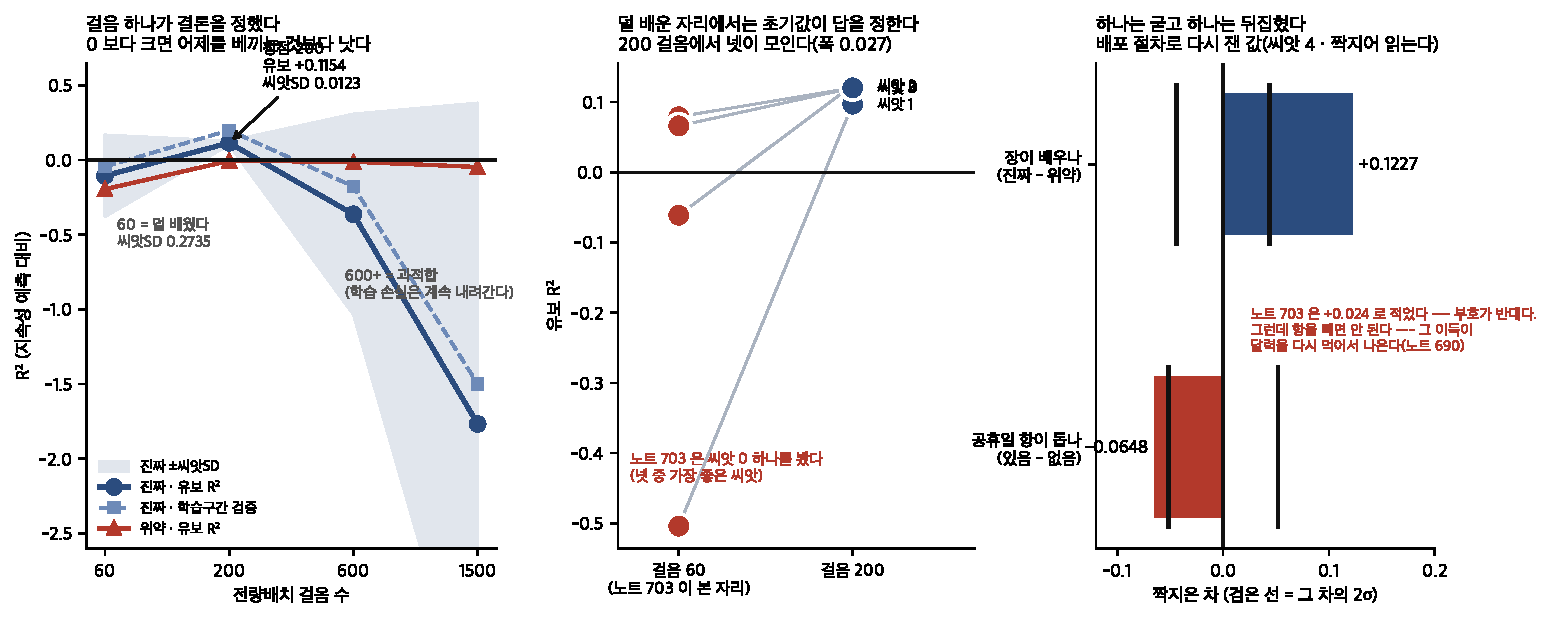
\includegraphics[width=0.99\textwidth]{figs/onestep.pdf}
\caption{왼쪽: \textbf{걸음 하나가 결론을 정했다} --- $60$ 은 덜 배웠고 $600$ 이후는
과적합이며 $200$ 에서 씨앗이 모인다. $0$ 보다 크면 어제를 베끼는 것보다 낫다.
가운데: \textbf{덜 배운 자리에서는 초기값이 답을 정한다.} 오른쪽: \textbf{하나는
굳고 하나는 뒤집혔다} --- 검은 선이 그 짝 차의 $2\sigma$ 다.}
\end{figure}

\subsection*{미수렴이 아니라 미수렴 \emph{그리고} 과적합이다}

노트 $733$ 에서 나는 원인을 \emph{``전량배치 $60$ 걸음은 수렴이 아니다''}로
진단하고 \textbf{걸음을 늘리면 씨앗 SD 가 줄 것}이라 사전등록했다. \textbf{절반만
맞았다} --- $200$ 까지는 줄고($0.2735 \to 0.0123$) 그 뒤로 폭발한다($0.6717 \to
2.1503$). \textbf{학습 손실은 내내 내려간다}($0.00504 \to 0.00220$) --- 그것이
과적합의 증거다.

\claim{\textbf{걸음 수를 고정값으로 두면 안 된다.} 정점 전이면 초기값이 답을
정하고 정점 후면 과적합이 답을 정한다. 그래서 \texttt{pretrain} 을 고쳐
\textbf{학습 구간 검증으로 최선 지점을 잡고 그 가중으로 되돌린다} --- 유보를 보고
고르면 그 순간 유보가 아니다.}
{정점을 학습 구간 검증으로 고르는 것이 \emph{유보에서도} 정점인지는 보장이 없다.
실측으로 확인했다 --- 손으로 고른 $200$ 걸음이 유보 $+0.1154$ 이고 절차가 고른
것($220$ · $600$ · $320$ · $180$ 씨앗마다)이 \textbf{$+0.1200$} 이다. \textbf{두
값이 거의 같으므로 절차가 정직하게 작동한다.} 다만 씨앗 하나는 상한 $600$ 에
걸렸다 --- 상한을 올리면 그 씨앗은 더 갈 수 있고, 그 경우 값이 조금 달라진다.}

\section{배포되는 절차로 확인했다}

\begin{center}
\begin{tabular}{lrl}
\toprule
& 유보 $R^2$ & 씨앗별 \\
\midrule
\textbf{진짜 · 공휴일 있음} & $\mathbf{+0.1200}$ & $+0.0905$ · $+0.1290$ · $+0.1286$ · $+0.1318$ \\
위약 & $-0.0027$ & $+0.0001$ · $-0.0040$ · $-0.0003$ · $-0.0067$ \\
진짜 · 공휴일 없음 & $+0.1848$ & $+0.1941$ · $+0.1788$ · $+0.1811$ · $+0.1851$ \\
\midrule
\textbf{짝 차(진짜 $-$ 위약)} & $\mathbf{+0.1227}$ & $2\sigma = 0.0438$ $\to$ \textbf{$5.6\sigma$ 밖} \\
공휴일 이득(있음 $-$ 없음) & $-0.0648$ & $2\sigma = 0.0518$ $\to$ \textbf{$2\sigma$ 밖} \\
\bottomrule
\end{tabular}
\end{center}

\claim{\textbf{정보 전이장은 진짜 유보에서 지속성 예측을 이긴다.} 과제가
$X[t{+}30] - X[t]$ 라 \textbf{베끼기는 $0$점}이므로 $+0.1200$ 은 \textbf{다른 동네와
과거 무늬에서 실제로 정보를 얻는다}는 뜻이다. 씨앗 넷이 다 양수이고 위약이
$-0.0027$ 로 $0$ 에 붙는다.}
{\textbf{이것은 판 측정이 아니다.} 유보 $R^2$ 는 \emph{장 자신의 과제}에서 잰
것이고 가드는 \emph{``시험대는 판''}이다. \textbf{장이 실재한다는 것과 판이
움직인다는 것은 다른 문장이다} --- 채택 시험은 인코더 출력을 판 열로 넣어 신호
몫을 재고 규약 $12$(집안 $\geq 1$ · 집 밖 $\geq 2$)를 통과하는 것이고, 아직 안 했다.}

\subsection*{씨앗 잡음은 짝지어 읽어야 한다}

씨앗 $1$ 은 걸음 $60$ 에서 진짜가 $-0.5041$ 이고 \textbf{위약도 $-0.5927$} 이다 ---
두 팔이 같이 무너진다. 노트 $712$ 가 \emph{``진짜$\leftrightarrow$위약 씨앗별 상관
$+0.825$ 라 씨앗 SD 를 신뢰구간으로 읽으면 안 된다''}고 적었고, \textbf{여기서 그
경고가 값을 했다} --- 팔별 SD($0.2735$)로 읽으면 아무 결론도 안 나고 짝 차로
읽으면 $6.5\sigma$ 다.

\section{그리고 손잡이 하나가 예보와 식별을 맞바꾼다}

\textbf{공휴일 항을 빼면 유보 $R^2$ 가 $+0.1200 \to +0.1848$ 로 오른다}(짝 차
$-0.0648$ · $2\sigma$ 밖 · 두 측정에서 씨앗 $8/8$ 이 같은 방향). 노트 $703$ 은
반대로 \emph{``공휴일 항이 학습에 도움 $+0.024$ --- 명절이 신호가 아니라
잡음이었다''}고 적었다. \textbf{그 결론을 철회한다} --- $+0.024$ 는 학습구간 안 ·
씨앗 하나의 값이었다.

\textbf{그런데 기본값을 바꾸지 않는다.} 노트 $690$ 이 그 항을 넣은 이유가
예보가 아니었다.

\begin{center}
\begin{tabular}{lrr}
\toprule
& 공휴일 항 없음 & 공휴일 항 있음 \\
\midrule
유보 $R^2$ & $\mathbf{+0.1848}$ & $+0.1200$ \\
$g$ 큰 이상치의 \textbf{달력 귀속률}(광역) & $86.7\%$ & $\mathbf{48.3\%}$ \\
같은 것(동네) & $86.7\%$ & $\mathbf{61.7\%}$ \\
\bottomrule
\end{tabular}
\end{center}

\claim{\textbf{한 층의 예보 지표가 오르는 것이 다른 층의 식별을 깨면 개선이
아니다.} 공휴일 항을 빼서 얻는 $+0.065$ 는 \textbf{명절을 다시 먹어서} 나온다.
그러면 $g_{\text{지역}}$ 이 대부분 명절이 되어 \textbf{\texttt{cal\_*} 축의
재발견}이 된다 --- 노트 $690$ 이 정확히 그것을 막으려고 항을 넣었다. \textbf{그래서
장의 자는 유보 $R^2$ 하나가 아니라 (유보 $R^2$, 달력 귀속률) 짝이다.}}
{두 목표가 실제로 맞바꾸는지는 \textbf{한 팔에서 둘을 같이 재야} 확정된다 --- 이
논문은 $R^2$ 를 이번에 재고 귀속률을 노트 $690$ 에서 가져왔다. 같은 코드 · 같은
씨앗에서 둘을 같이 찍으면 맞바꿈 곡선이 나오고, 그때 \textbf{어느 지점을 고르나가
설계 결정}이 된다. 그 측정을 안 했다.}

\subsection*{노트 $703$ 이 왜 틀렸나 --- 자가 하나였기 때문이다}

노트 $703$ 은 $R^2$ 만 보고 공휴일 항을 칭찬했다. \textbf{그 층에 자가 하나뿐이라
맞바꿈이 안 보였다.} 이것은 노트 $715 \cdot 717$ 이 문턱을 눈금한 것과 같은 층의
일이고, 논문 $142$ 가 세운 조항(\emph{``신호 몫을 보고할 때 축 품질을 같이
적는다''})과도 같은 모양이다 --- \textbf{자를 하나만 두면 그 자가 오르는 방향으로
설계가 끌려간다.}

\section{사전등록 채점}

\begin{center}
\begin{tabular}{llll}
\toprule
& 예측 & 실측 & \\
\midrule
노트 $732$ ① & 유보 $R^2$ $0.02 \sim 0.10$ & $-0.1051$ & \textbf{틀림} \\
노트 $732$ ⑤ & 씨앗 SD $0.01 \sim 0.03$ & $\mathbf{0.2735}$ & \textbf{열 배 틀림} \\
노트 $734$ ① & $1500$ 걸음에서 SD $<0.05$ & $2.1503$ & \textbf{틀림}(정점에서는 맞다) \\
노트 $734$ ② & 유보 $0.05 \sim 0.15$ 양수 & $+0.1154$ & \textbf{맞음} \\
노트 $734$ ③ & 짝 차 $0.09 \sim 0.20$ & $+0.1208$ & \textbf{맞음} \\
노트 $734$ ④ & 손실이 $600$ 안에 평탄 & 계속 내려간다 & \textbf{틀림} \\
노트 $734$ ⑤ & 위약이 $|0.03|$ 안 & $-0.0054$ & \textbf{맞음} \\
\bottomrule
\end{tabular}
\end{center}

\textbf{가장 크게 틀린 것이 씨앗 SD 예측($0.01{\sim}0.03$ 대 실측 $0.2735$)이고
그것이 이 사이클의 배움이다} --- \textbf{잡음을 안 재고 효과를 보고했으면 노트 703
과 같은 문장을 또 썼을 것이다.}

\end{document}
